\usetikzlibrary{calc}
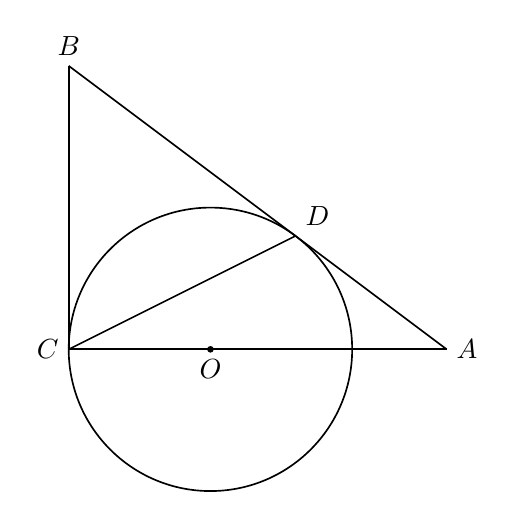
\begin{tikzpicture}[x=1cm,y=1cm,line width=.6pt,font=\normalsize]
\coordinate (O) at (0.0,0.0);
\coordinate (C) at (-1.8,0.0);
\coordinate (A) at (3.0,0.0);
\coordinate (B) at (-1.8,3.6);
\coordinate (D) at (1.08,1.44);
\draw (O) circle[radius=1.8cm];
\draw (B)--(C);
\draw (C)--(A);
\draw (B)--(A);
\draw (C)--(D);
\fill (O) circle[radius=1.2pt];
\node[above] at (B) {$B$};
\node[left] at (C) {$C$};
\node[right] at (A) {$A$};
\node[above right] at (D) {$D$};
\node[below] at (O) {$O$};
\end{tikzpicture}
